\section{Transformation to Polygonal Dual}
\label{sect:transformation-to-polygonal-dual}

In this step of the pipeline, we take an embedded cluster graph $G_\text{emb}$ and form a polygonal dual of $G_\text{emb}$, our initial map graph $G_\text{init}$.

Let us discuss the relationship between $G_\text{emb}$ and $G_\text{init}$ a bit more. Recall from \cref{chap:preliminaries} that the weak dual of a plane graph is its dual without the vertex corresponding to its outer face. Using this terminology, given $G_\text{init}$, which is a hole-free polygonal dual of the plane graph $G_\text{emb}$, we can smooth out the degree-2 vertices in $G_\text{init}$ and form its weak dual to get back $G_\text{emb}$, as illustrated in the following figure:
%
\begin{figure}[H]
	\centering
	\subfigure[]{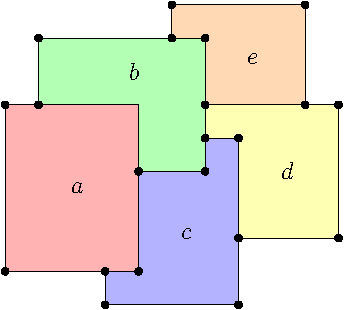
\includegraphics[height=90px]{Resources/StaticPipeline-RectilinearDual-Dual.pdf}\label{fig:static-pipeline-rectilinear-dual-dual}}
	\quad
	\subfigure[]{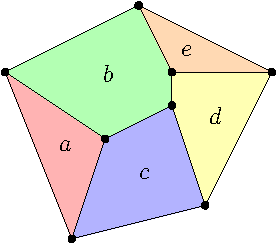
\includegraphics[height=90px]{Resources/StaticPipeline-RectilinearDual-DualSmoothed.pdf}\label{fig:static-pipeline-rectilinear-dual-dual-smoothed}}
	\quad
	\subfigure[]{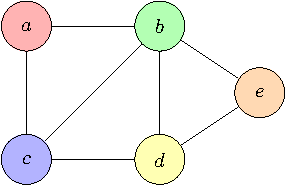
\includegraphics[height=90px]{Resources/StaticPipeline-RectilinearDual-Primal.pdf}\label{fig:static-pipeline-rectilinear-dual-primal}}
	\caption{A polygonal dual $G_\text{init}$ of some plane graph $G_\text{emb}$ (a), $G_\text{init}$ with its degree-2 vertices smoothed out (b), and the smoothed graphs's weak dual, $G_\text{emb}$ again (c).}
	\label{fig:static-pipeline-rectilinear-dual}
\end{figure}

We can also formalize the other direction, namely how to get from \cref{fig:static-pipeline-rectilinear-dual-primal} back to \cref{fig:static-pipeline-rectilinear-dual-dual}. To do so, we need the concept of an augmented dual:
%
\begin{definition}
	The \emph{augmented dual} $G^+$ of a plane graph $G$ is the plane multigraph obtained by first placing a new vertex in the outer face of $G$, connecting it to all vertices on the outer face, in order, without introducing edge crossings, and then forming its dual.
\end{definition}

\Cref{fig:static-pipeline-augmented-dual} illustrates how the augmented dual is formed.
%
\begin{figure}[H]
	\centering
	\subfigure[]{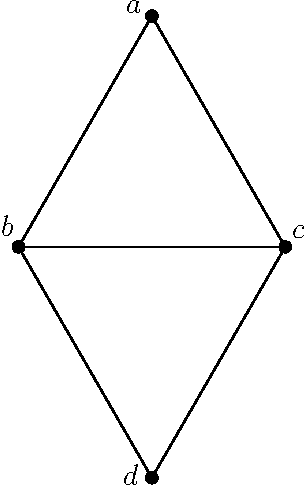
\includegraphics[height=90px]{Resources/StaticPipeline-AugmentedDual-1.pdf}}
	\quad
	\subfigure[]{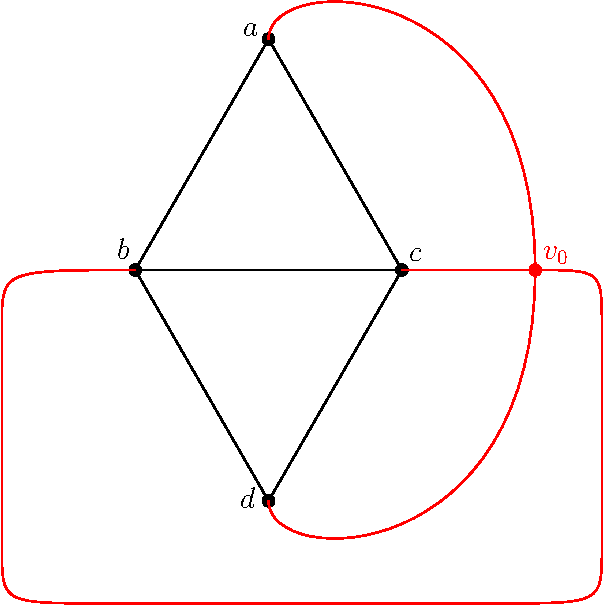
\includegraphics[height=90px]{Resources/StaticPipeline-AugmentedDual-2.pdf}}
	\quad
	\subfigure[]{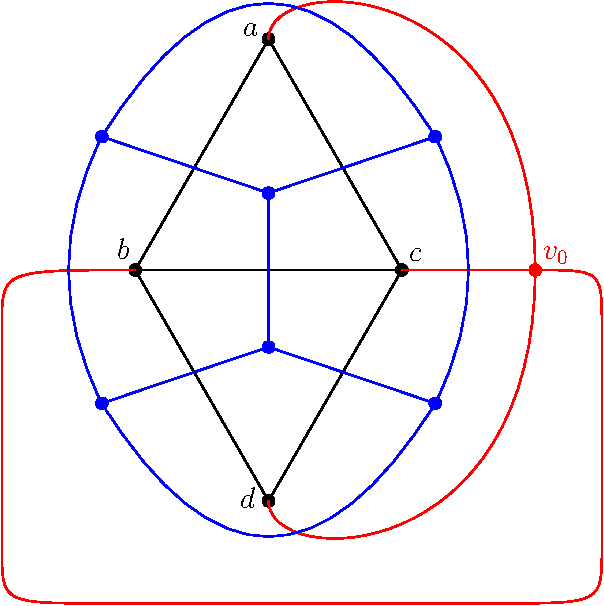
\includegraphics[height=90px]{Resources/StaticPipeline-AugmentedDual-3.pdf}}
	\quad
	\subfigure[]{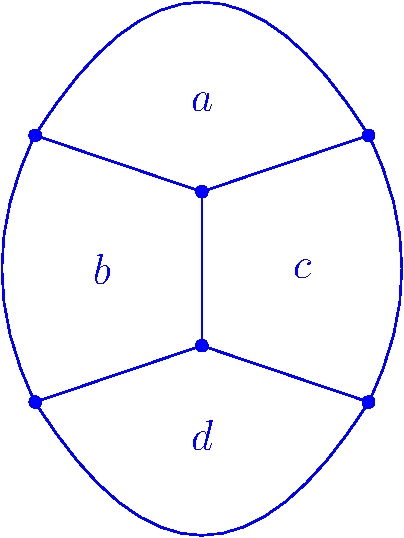
\includegraphics[height=90px]{Resources/StaticPipeline-AugmentedDual-4.pdf}}
	\caption{Step-by-step representation of forming a plane graph $G$ (a)'s augmented dual. We add the helper vertex in the outer face in red (b) and form the regular dual in blue (c). (d) shows just the augmented dual $G^+$.}
	\label{fig:static-pipeline-augmented-dual}
\end{figure}

Note that analogous the regular dual, the weak dual of the augmented dual of a plane graph $G$ is $G$ again, \ie{} $(G^+)^- = G$. With this definition in plane, we make the following observation:

\begin{corollary}
	A polygonal dual of an internally triangulated plane graph $G$ is a straight-line planar embedding of a subdivision of its augmented dual $G^+$.
\end{corollary}


\paragraph{Theoretical Results}

But do we have to subdivide edges of the augmented dual of our embedded cluster graph $G_\text{emb}$ in order to get a valid polygonal dual of $G_\text{emb}$? Although the augmented dual $G_\text{emb}^+$ is plane by definition, it is not immediately obvious that there exists a planar straight-line embedding of $G_\text{emb}^+$ \emdash{} and that's what we need for it to be a polygonal contact representation.

In our case, however, $G_\text{emb}^+$ is simple, \ie{} there are no loops or multiple adjacencies. Recall that $G_\text{emb}$ is 2-connected and internally triangulated. Adding the helper vertex in the outer face of $G_\text{emb}$ and connecting it to all vertices on the outer face therefore creates a fully triangulated, simple graph. In a simple triangulated graph, there are no two edges that are incident to the same faces (only those would create multiple adjacencies when forming the dual) and no edges that have the same face on both sides (only those would create loops when forming the dual) either. The augmented dual $G_\text{emb}^+$ is therefore simple and, according to Fáry's theorem \cite{fary1948straight}, there exists a planar straight-line embedding of $G_\text{emb}^+$ respecting its original combinatorial embedding.

In addition to having a planar straight-line embedding, $G_\text{emb}^+$ is also a cubic graph, \ie{} one in which all vertices have degree 3. This is because $G_\text{emb}$ with the helper vertex is a triangulated graph, meaning every face is incident to exactly three edges, which turns into every vertex being incident to exactly three edges when forming the dual. According to the results of Thomassen \cite{thomassen1992plane}, $G_\text{emb}^+$ is therefore area-universal. This means that regardless of the concrete face weights that $G_\text{emb}$ prescribes, there exists a planar straight-line embedding of $G_\text{emb}^+$ realizing those weights/areas.

Even without subdividing edges in $G_\text{emb}^+$, we could therefore choose the initial map graph $G_\text{init}$ in such a way that it has perfect statistical accuracy already. Such an embedding of $G_\text{emb}^+$ is non-trivial to compute though and creates undesired region shapes according to our other quality metrics. Instead, we provide a very simple algorithm that subdivides all edges of the augmented dual once and leaves us with enough degrees of freedom to optimize for other quality metrics in \cref{sect:drawing-the-polygonal-dual}.


\paragraph{Algorithm Overview}

The underlying idea is as follows: Given an embedded cluster graph $G_\text{emb}$, we place vertices on edges of the outer face of $G_\text{emb}$ (those edges bound additional triangular faces after adding the helper vertex in the process of forming the augmented dual) and inside the internal faces of $G_\text{emb}$. We then connect these vertices if their corresponding faces are incident. Connecting two vertices may require additional subdivision vertices in order not to introduce edge crossings \emdash{} we use a single subdivision vertex per edge.

% and was independently proved by Wagner \cite{wagner1936bemerkungen} and Stein \cite{stein1951convex}.
In a preliminary step, we tweak the embedding of $G_\text{emb}$ to use straight-line edges. As mentioned before, such an embedding exists for every plane graph according to Fáry's theorem \cite{fary1948straight}. There exist numerous popular algorithms to construct such an embedding such as Tutte's method \cite{tutte1963draw}, the shift method \cite{fraysseix1990draw}, or the Schnyder realizer method \cite{schnyder1990embedding}. \tamara{is this Tutte the algorithm with exponential area you meant?}


\clearpage
\paragraph{Algorithm Implementation}

\begin{algorithm}[H]
  \caption{Transformation to Polygonal Dual}
  \label{algo:transformation-to-dual}
  \SetKwData{Endpoints}{endpoints}
  \SetKwFunction{Appending}{appending}
  \SetArgSty{textrm}
  \vspace{5pt}
  \KwData{planar straight-line embedding of 2-connected, internally triangulated graph $G_\text{emb}$}
  \KwResult{planar straight-line embedding of 1-subdivision of augmented dual $G_\text{init}$ of $G_\text{emb}$}
  \vspace{10pt}
  create empty output graph $G_\text{out}$\;
  \ForEach{inner face $f$ in $G_\text{in}$}{
    \label{line:transformation-loop1-start}
    add \quoted{inner face vertex} $v_f$ to $G_\text{out}$\;
    position $v_f$ at barycenter of $f$ in $G_\text{in}$ \label{line:transformation-barycenter1}\;
    \label{line:transformation-loop1-end}
  }
  \ForEach{edge $\{u,v\}$ in $G_\text{in}$}{
    \label{line:transformation-loop2-start}
  	\If{$\{u,v\}$ is incident to two different internal faces $f, g$ in $G_\text{in}$ \label{line:transformation-incidentfacelookup1}}{
  	  add \quoted{subdivision vertex} $v_\text{sub}$ to $G_\text{out}$\;
  	  position $v_\text{sub}$ at midpoint of ${\{u,v\}}$ in $G_\text{in}$\;
  	  add edge between $v_f$ and $v_\text{sub}$ to $G_\text{out}$\;
  	  add edge between $v_\text{sub}$ and $v_g$ to $G_\text{out}$\;
  	}
  	\ElseIf{$\{u,v\}$ is incident to a single internal face $f$ in $G_\text{in}$ \label{line:transformation-incidentfacelookup2}}{
  	  add \quoted{outer edge vertex} $v_{\{u,v\}}$ to $G_\text{out}$\;
  	  position $v_{\{u,v\}}$ at midpoint of ${\{u,v\}}$ in $G_\text{in}$\;
  	  add \quoted{subdivision vertex} $v_\text{sub}$ to $G_\text{out}$\;
  	  position $v_\text{sub}$ at midpoint of barycenter of $f$ and midpoint of ${\{u,v\}}$ in $G_\text{in}$ \label{line:transformation-barycenter2}\;
  	  add edge between $v_{\{u,v\}}$ and $v_\text{sub}$ to $G_\text{out}$\;
  	  add edge between $v_\text{sub}$ and $v_f$ to $G_\text{out}$\;
  	}
  	\label{line:transformation-loop2-end}
  }
  \ForEach{incident edges $\{\{u,v\},\{v,w\}\}$ on outer face of $G_\text{in}$}{
    \label{line:transformation-loop3-start}
    add \quoted{subdivision vertex} $v_\text{sub}$ to $G_\text{out}$\;
    position $v_\text{sub}$ at position of $v$ in $G_\text{in}$\;
    add edge between $v_{\{u,v\}}$ and $v_\text{sub}$ to $G_\text{out}$\;
    add edge between $v_\text{sub}$ and $v_{\{v,w\}}$ to $G_\text{out}$\;
    \label{line:transformation-loop3-end}
  }
  \ForEach{vertex $u$ in $G_\text{in}$ \label{line:transformation-enumeratevertices}}{
    \label{line:transformation-loop4-start}
    $\Endpoints \gets ()$\;
    \ForEach{adjacent pair $(v,w)$ of neighbors of $u$ (according to embedding) \label{line:transformation-enumerateedges}}{
      \If{$u,v,w$ is a triangular face $f$ with positive area in $G_\text{in}$ \label{line:transformation-checktriangle}}{
        append $v_f$ to \Endpoints\;
      }
      \Else{
        append $v_{\{u,v\}}$ to \Endpoints\;
        append $v_{\{u,w\}}$ to \Endpoints\;
      }
    }
    \ForEach{adjacent pair $(v,w)$ in \Endpoints}{
      insert subdivision vertex connecting $v$ to $w$ between $v$ and $w$ in \Endpoints\;
    }
    define $f_u$ as face on \Endpoints\;
    set weight of $f_u$ to weight of $u$ in $G_\text{in}$\;
    \label{line:transformation-loop4-end}
  }
  \ForEach{edge $\{u,v\}$ in $G_\text{in}$}{
    \label{line:transformation-loop5-start}
    set weight of adjacency between $f_u$ and $f_v$ to weight of $\{u,v\}$ in $G_\text{in}$\;
    \label{line:transformation-loop5-end}
  }
  \Return $G_\text{out}$
\end{algorithm}
\vfill

\paragraph{Algorithm Correctness}
\lipsum

\begin{figure}[H]
	\centering
	\subfigure[$G_\text{in}$]{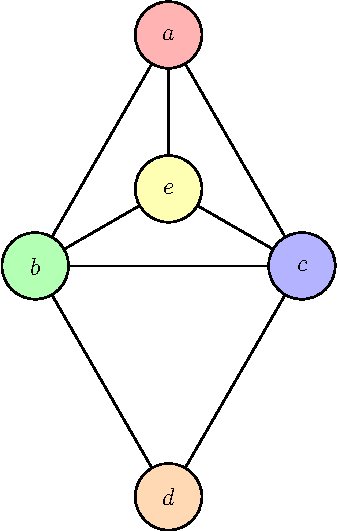
\includegraphics[height=70mm]{Resources/Implementation-Transformation-Primal.pdf}}
	\quad
	\subfigure[$G_\text{out}$]{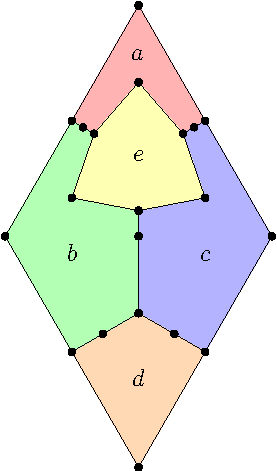
\includegraphics[height=70mm]{Resources/Implementation-Transformation-Dual.pdf}}
	\caption{An embedded filtered graph (a) and its dual as produced by \cref{algo:transformation-to-dual} (b).}
	\label{fig:implementation-transformation}
\end{figure}

\paragraph{Algorithm Runtime}

To compute the input graph's faces, we replace every edge with two inversely oriented, directed edges. We then repeatedly pick any unmarked edge and form a directed cycle by following the next outgoing edge according to the embedding, marking the edges as we go. Once all edges have been marked, we have found all faces. The outer face is the only face with negative area. This can be implemented in $\bigTheta{\abs{V_\text{in}} + \abs{E_\text{in}}}$.

The input graph has $\bigTheta{\abs{V_\text{in}}}$ internal faces and they are all triangles, therefore we can compute their barycenter in $\bigTheta{1}$ each (\cref{line:transformation-barycenter1}, \cref{line:transformation-barycenter2}). By keeping track of of which faces an edge of the input graph is incident to while computing the faces as outlined above, we allow for $\bigTheta{1}$ lookups in \cref{line:transformation-incidentfacelookup1} and \cref{line:transformation-incidentfacelookup2}. The loop in \crefrange{line:transformation-loop1-start}{line:transformation-loop1-end} therefore runs in $\bigTheta{\abs{V_\text{in}}}$, the loop in \crefrange{line:transformation-loop2-start}{line:transformation-loop2-end} in $\bigTheta{\abs{E_\text{in}}}$, and the loop in \crefrange{line:transformation-loop3-start}{line:transformation-loop3-end} in $\bigTheta{\abs{E_\text{in}}}$.

The loop in \crefrange{line:transformation-loop4-start}{line:transformation-loop4-end} processes every vertex once in \cref{line:transformation-enumeratevertices} and and every edge twice \cref{line:transformation-enumerateedges}. We can check if the vertices $u,v,w$ form a triangle in constant time (\cref{line:transformation-checktriangle}) by checking if there's an edge between $v$ and $w$. Considering each of the $\bigTheta{\abs{V_\text{in}} + \abs{E_\text{in}}}$ vertices of the generated graph appears in \code{endpoints} in no more than two iterations of the loop in \crefrange{line:transformation-loop4-start}{line:transformation-loop4-end} and all those vertices have degree 3, we can find their shared neighbor in constant time and implement the entire loop to run in $\bigTheta{\abs{V_\text{in}} + \abs{E_\text{in}}}$.

By keeping track of which faces in the generated graph correspond to which vertices in the source graph in \crefrange{line:transformation-loop4-start}{line:transformation-loop4-end}, the loop in \crefrange{line:transformation-loop5-start}{line:transformation-loop5-end} runs in $\bigTheta{\abs{V_\text{in}} + \abs{E_\text{in}}}$.

The entire algorithm can therefore be implemented to run in $\bigTheta{\abs{V_\text{in}} + \abs{E_\text{in}}}$.
